%% HKUST unofficial poster template
% By Ching Ting Leung, class of 2025 in BEng

% Forked from Gemini theme
% https://github.com/anishathalye/gemini

% Required Compiler: pdfLaTeX (compatible with Overleaf)

\documentclass[final]{beamer}

% ====================
% Packages
% ====================

\usepackage[T1]{fontenc}
% \usepackage{lmodern}
% \usepackage{carter}
\usepackage{lmodern}
% \usepackage{sansmathfonts}
% \renewcommand{\familydefault}{\sfdefault}
% \usepackage[size=custom,width=60in,height=36in,scale=1.0]{beamerposter} % default
\usepackage[size=custom,width=152.4,height=91.44,scale=1.35]{beamerposter} % default
% \usepackage[orientation=landscape,size=a0,scale=1.4]{beamerposter} % custom
% scale: scaling factor of all font


\newcommand{\sumgraph}{\underset{n \in [N]}{\sum}}
\def \sumneighbors {\underset {m\in{\mathcal{N}(n)}}{\sum}}

\def \sumstrangers{\underset {m\notin{\mathcal{N}(n)}}{\sum}}
\def \sumgraphu {\underset{n\in [N]}{ \sum}}


\usetheme{gemini}
\usecolortheme{Tuebingen} % Customize in beamercolorthemeTuebingen.sty

\usepackage{graphicx}
\usepackage{booktabs}
\usepackage{tikz}
\usetikzlibrary{calc}
\usepackage{pgfplots}
\pgfplotsset{compat=1.14}
\usepackage{anyfontsize}

% ====================
% Lengths
% ====================
%
% If you have N columns, choose \sepwidth and \colwidth such that
% (N+1)*\sepwidth + N*\colwidth = \paperwidth
\newlength{\sepwidth}
\newlength{\colwidth}
\setlength{\sepwidth}{0.02\paperwidth}
\setlength{\colwidth}{0.220\paperwidth}
% \setlength{\sepwidth}{0.025\paperwidth}
% \setlength{\colwidth}{0.3\paperwidth}

\newcommand{\separatorcolumn}{\begin{column}{\sepwidth}\end{column}}

% ====================
% Title
% ====================

\title{PieClam: Inclusive Exclusive Cluster Affiliation Model With Prior}

\author{Daniel Zilberg, Ron Levie}

% \institute[shortinst]{\inst{1} Department of Chemical and Biological Engineering, Hong Kong University of Science and Technology \and \inst{2} Department of Computer Science and Engineering, Hong Kong University of Science and Technology}

% ====================
% Footer (optional)
% ====================

% \footercontent{
%   \href{https://www.example.com}{https://www.example.com} \hfill
%   ABC Conference 2025, Hong Kong --- XYZ-1234 \hfill
%   \href{mailto:youremail}{youritsc12@connect.ust.hk}}
% (can be left out to remove footer)

% ====================
% Logo (optional)
% ====================

% use this to include logos on the left and/or right side of the header:
\logoleft{
\includegraphics[height=6cm]{images/ICML-logo.png}}
\logoright{
\includegraphics[height=9cm]{images/QR_archive.png} \hspace{1cm} 
\includegraphics[height=9cm]{technion logo.png}}

% ====================
% Body
% ====================

% Custom column title style
\newcommand{\columntitle}[1]{
  \vspace{1em}
  \begin{center}
    \color{white}
    \fcolorbox{black}{blue!80!black}{\parbox{0.9\columnwidth}{\centering\LARGE\bfseries #1}}
  \end{center}
  \vspace{1em}
}

\begin{document}

\begin{frame}[t]

\begin{columns}[t]
\separatorcolumn

\begin{column}{\colwidth}
  \columntitle{Background}
  \begin{block}{Graph Representation Learning}
    \textbf{Setting}: An \textbf{undirected, featureless} \textbf{graph} $G = ([N], E)$ with an adjacency matrix $\mathbf{A}= \{a_{nm}\in \{0,1\}\}_{n,m = 1}^N$. 
          An edge between nodes $n$ and $m$ is denoted by $n\sim m$. A non-edge by $n\not\sim m$.
    
        % \item A Random Graph Model is An $N\times N$ matrix with elements $p_{nm} = P(n\sim m)$
        
    \textbf{Goal}:
    % \vspace{-0.8em}
    Build a \textbf{universal autoencoder}, which can represent any graph $G$ of any size $N$ with a fixed budget of parameters per node $C$.
    % \end{itemize}
  \end{block}

  \begin{block}{BigClam \cite{yang2013overlapping}: Inclusive Community Affiliation}
    \textbf{Inclusive communities}: 
    Common membership raises the probability to connect: $P(n\sim m \big| \mathbf{f}_n, \mathbf{f}_m) = 1-e^{-\mathbf{f}_n^\top \mathbf{f}_m}$
    % Edges are decoded from a Poisson distribution over the inner product between features: $P(n\sim m \big| \mathbf{f}_n, \mathbf{f}_m) = 1-e^{-\mathbf{f}_n^\top \mathbf{f}_m}$
    
    The probability for the entire graph is
         % PAIRS ARE INDEPENDENT
         \[ P(E|\mathbf{F}) = \sqrt{\prod_{n \in [N]}\prod_{m \in \mathcal{N}(n)}P( n\sim m|\mathbf{\mathbf{f}_n, \mathbf{f}_m})\prod_{m \notin \mathcal{N}(n)} P( n\not\sim m)|\mathbf{f}_n, \mathbf{f}_m)}\]%\pause
         
    The log likelihood is 
    \[ l(\mathbf{F}) = \frac{1}{2}\sumgraph \Big(\sumneighbors{}{\log(1-e^{-\mathbf{f}_n^{\top } \mathbf{f}_m})} - 
    \sumstrangers{\mathbf{f}_n^{\top } \mathbf{f}_m}\Big).\]%\pause
    Optimize with gradient updates  
        \[ \nabla_{\mathbf{f}_n}l = 
            \sumneighbors{\mathbf{f}_m \big(1-e^{-\mathbf{f}_n^\top  \mathbf{f}_m}
            \big)^{-1}} - \sumgraph{\mathbf{f}_m} + \mathbf{f}_n .\]%\pause
    Can be implemented as an \textbf{MPNN}.
    
    
  \end{block}

  \begin{alertblock}{Bipartite Blindness Of BigClam}
  
    \begin{figure}
        \begin{minipage}{0.35\columnwidth}
        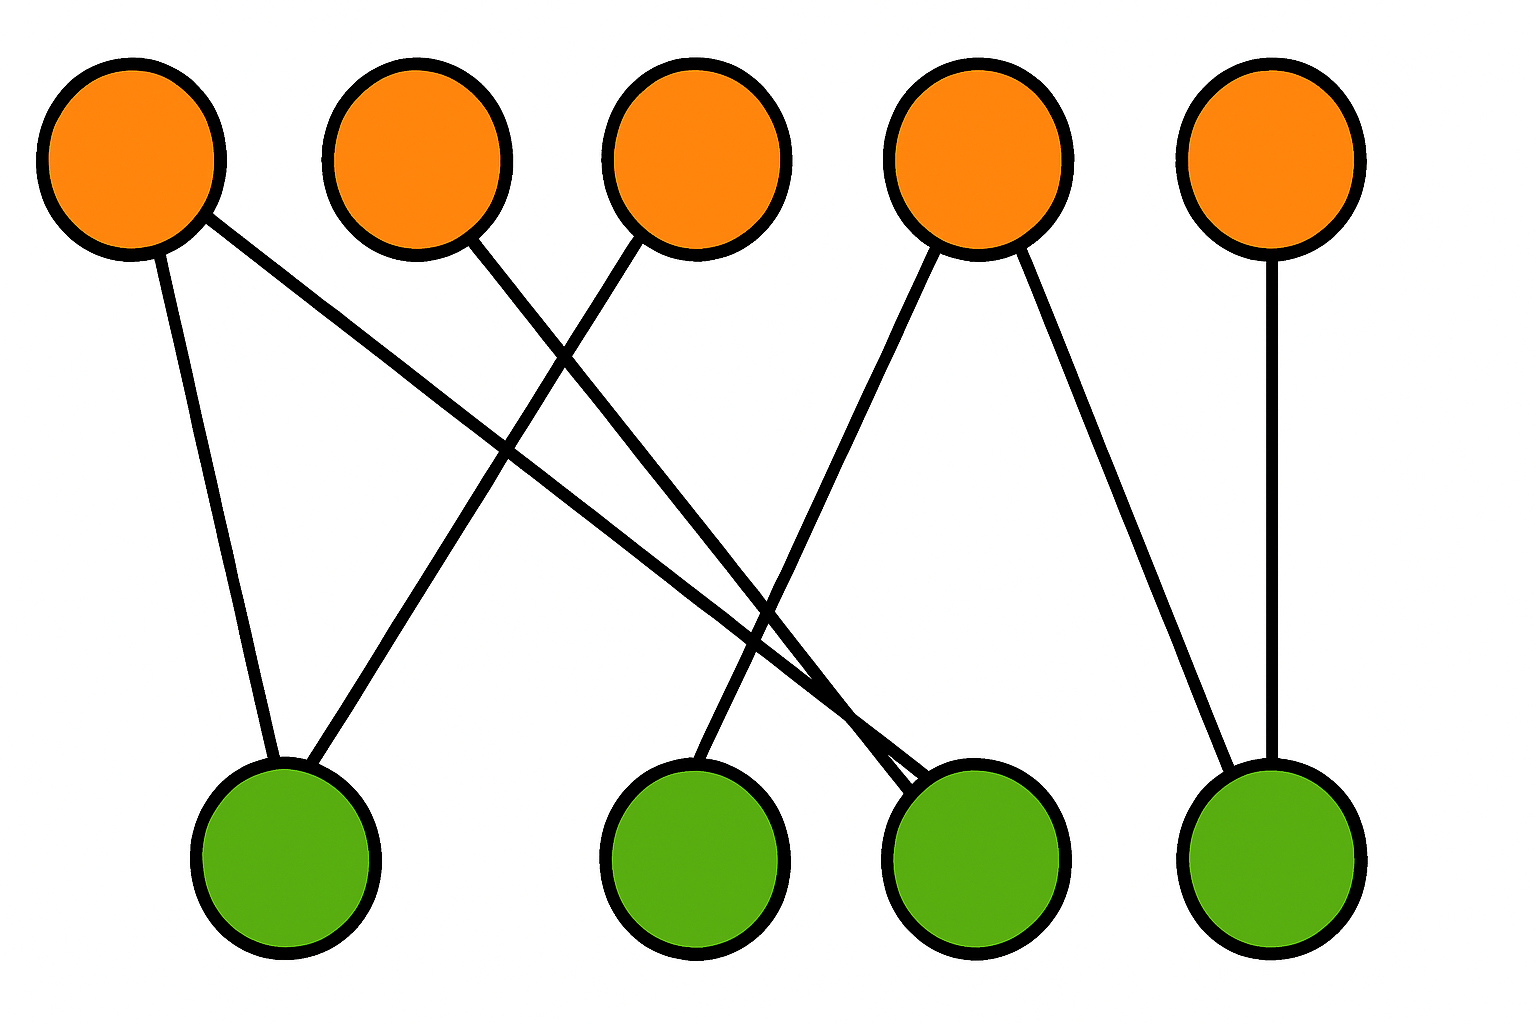
\includegraphics[width=\textwidth]{images/bipart/bipart_pic_orange_red.png}    
        \end{minipage} \hspace{3em} 
        \begin{minipage}{0.25\columnwidth}
            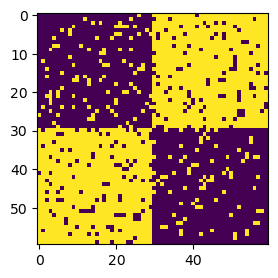
\includegraphics[width=\textwidth]{images/bipart/bipart_gt_30nodes.png}
        \end{minipage}
        
    \end{figure}
    \textbf{Triangle inequality}: if $n\sim k$ and $m\sim k$ then $\mathbf{f}_{n}^\top \mathbf{f}_k$ and $\mathbf{f}_{m}^\top \mathbf{f}_k$ are large and therefore $\mathbf{f}_n^\top \mathbf{f}_m$ is also large which implies $m\sim n$ with high probability.%\pause
    \begin{figure}    
        \begin{minipage}{0.27\columnwidth}
            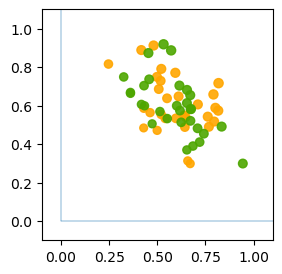
\includegraphics[width=\textwidth]{images/bipart/embedding_bc_best.png}
        \end{minipage}
        \hspace{3em}
        \begin{minipage}{0.30\columnwidth}
        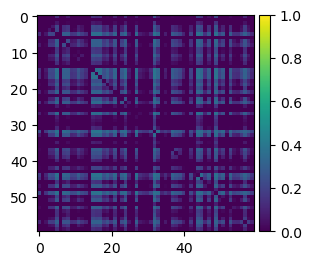
\includegraphics[width=\textwidth]{images/bipart/decode_bc_30nodes.png}       
        \end{minipage}\hfill
        \caption{Bipartite autoencoding with BigClam}
    \end{figure}
  
  \LARGE{Inner product decoding is not universal!}

  
  \end{alertblock}
\vspace{-0.8em}
  \LARGE{Quick fix: \fcolorbox{blue!60}{blue!10}{\textbf{use node features!}} or...}
\end{column}

\separatorcolumn

\begin{column}{\colwidth}
  \columntitle{Innovations}
  \begin{block}{IeClam: Inclusive Exclusive Clustering}

    \textbf{Exclusive communities}: common membership \textit{reduces} the probability to connect.
    
    \textbf{Representation}: $\mathbf{f}_n = (\mathbf{t}_n, \mathbf{s}_n)$ where $\mathbf{t}_n$ are inclusive and $\mathbf{s}_n$ are exclusive communities.
    
    \textbf{L-Product}: Instead of inner product use
    \[\mathbf{f}_n^\top \mathbf{L} \mathbf{f}_m = \mathbf{t}_n^\top \mathbf{t}_m - \mathbf{s}_n^\top \mathbf{s}_m\]
    where $\mathbf{L} = {\rm diag}(1,\dots, 1, -1, \dots, -1)$.
    
    \textbf{Edge probability}:
    \[P(n \sim m| \mathbf{f}_n, \mathbf{f}_m) = 1-e^{-\mathbf{f}_n^\top \mathbf{L} \mathbf{f}_m}\]
    
    \textbf{Log likelihood}:
    \[ l(\mathbf{F}) = \frac{1}{2}\sumgraph \Big(\sumneighbors{}{\log(1-e^{-\mathbf{f}_n^\top \mathbf{L} \mathbf{f}_m})} - 
 \sumstrangers{\mathbf{f}_n^\top \mathbf{L} \mathbf{f}_m}\Big)\]

    % \textbf{Pairwise cone space $\mathcal{T}^C$}: Restrict $\mathbb{R}^{2C}$ to pairwise cones
    % \[\mathcal{T} = \{\mathbf{f}=(\mathbf{t}, \mathbf{s}) \text{ \textbf{s.t.} } \forall c\in[C]: |s^c| \leq t^c\}\]
    % This ensures positive probabilities and allows $(s^c,t^c)$ to be interpreted as complex features.

    \textbf{Bipartite encoding}: A bipartite graph can be encoded by embedding part 1 to $(b,b)$ and part 2 to $(b,-b)$ where $b\in \mathbb{R}_+$.

    \begin{figure}
      \centering
      \begin{minipage}{0.31\columnwidth}
        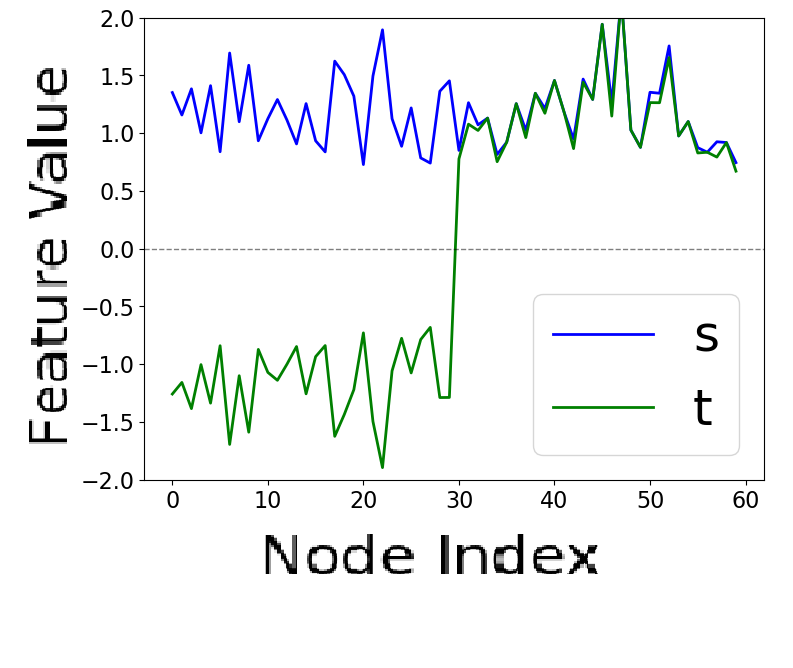
\includegraphics[width=\textwidth]{images/bipart/feat_vs_node_narrow_bigfont.png}
      \end{minipage}
      \hspace{0.05\columnwidth}
      \begin{minipage}{0.25\columnwidth}
        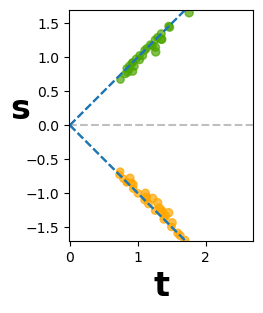
\includegraphics[width=\textwidth]{images/bipart/ieclam_cone_30nodes.png}
      \end{minipage}
      \hspace{0.05\columnwidth}
              \begin{minipage}{0.3\columnwidth}
          \raisebox{1.5em}{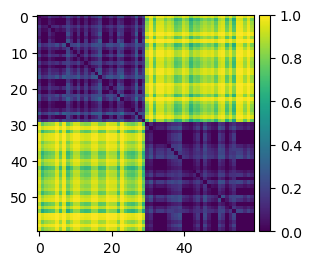
\includegraphics[width=\textwidth]{images/bipart/decode_ie_30nodes.png}}
        \end{minipage}
      \caption{Bipartite encoding with IeClam. \textbf{Left}: community value per node. \textbf{Center}: embedding space with one $\mathbf{s}$ and one $\mathbf{t}$ community, \textbf{Right}: reconstucted adjacency.}
    \end{figure}

  \end{block}

  \begin{block}{PieClam}

    Extend BigClam and IeClam into \textbf{Generative models}: Learn a joint probability distribution 
    \[p(E\wedge \mathbf{F}) = P(E|\mathbf{F})p(\mathbf{F})\]
    
    % Independent Features: 
    % \[p(\mathbf{F}) = \prod_{n\in[N]}p(\mathbf{f}_n)\]
    
    \textbf{Log likelihood loss} (assuming independent features):
    \[l(\mathbf{F})=
   \sumgraphu \Bigg(\frac{1}{2}\Big(\sumneighbors{\log(e^{\mathbf{f}_n^\top  \mathbf{L} \mathbf{f}_n} - 1)}  - \mathbf{f}_n^\top \mathbf{L} {\sumgraph{\mathbf{f}_m}} + \mathbf{f}_n^\top \mathbf{L} \mathbf{f}_n \Big) + \log\big(p(\mathbf{f}_n)\big)\Bigg)\]
   \textbf{Neural network prior}: Model $p(\mathbf{F})$ as a \textbf{normalizing flow} \cite{dinh2016density}.
  
   \textbf{Optimization}: Alternating optimization between features and prior parameters.
   
   \textbf{PClam}: Extend BigClam into a generative model by the same method.
  \end{block}
  
  \textbf{Graph Generation}: Sample N affiliation vectors from the prior and connect with $P(E|\mathbf{F})$
\end{column}

\separatorcolumn

\begin{column}{\colwidth}
  \columntitle{Theory}
  \begin{exampleblock}{Universality in Autoencoders}

     A family of code spaces $\{\mathbb{R}^C\}_{C\in\mathbb{N}}$ and corresponding decoders \\ $\{\mathbf{D}_C:\mathbb{R}^{2C}\rightarrow[0,1]^{N\times N}\}_{C\in\mathbb{N}}$ is \textbf{universal} w.r.t. to the distance $d(.,.)$ if for every $\epsilon>0$ there is $C\in\mathbb{N}$ (depending only on $\epsilon$) such that for every $N\in\mathbb{N}$ and every graph with adjacency matrix $\mathbf{A}\in[0,1]^{N\times N}$ there are $N$ points $\{z_n\in\mathbb{R}^C\}_{n=1}^N$ such that 
     \[d(\mathbf{D}_M(\mathbf{z}), \mathbf{A}) <\epsilon.\]

 

  \end{exampleblock}
  % \begin{figure}
  %     \centering
  %     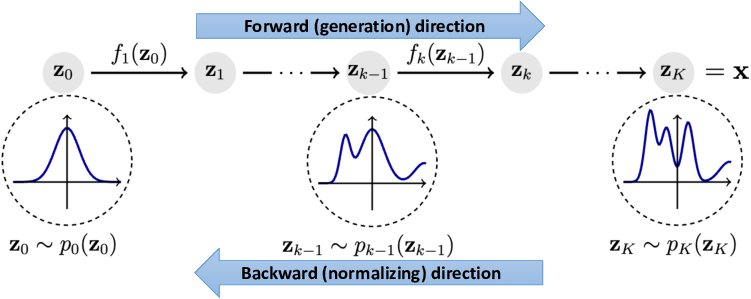
\includegraphics[width=0.8\linewidth]{images/normflow.png}
  %     \caption{Normalizing flow prior architecture}
  % \end{figure}

  % \vspace{1em}

  \begin{block}{Log Cut Distance}

    \textbf{Log Cut Metric} between probabilistic graph models:
    \[
        D_{\square}(\mathbf{P} || \mathbf{Q}):=  \frac{1}{N^2}\sup_{\mathcal{U},\mathcal{V}\subset[N]}\Bigg(\Big|\log\Big(\prod_{n\in \mathcal{U}}\prod_{m\in \mathcal{V}}
\frac{1-p_{n,m}}{1-q_{n,m}}\Big)\Big|\Bigg)\]
    \[= \|\log(1-\mathbf{P})- \log(1-\mathbf{Q}) \|_{\square}\]
    
    \textbf{Interpretation}: The biggest part of the probabilistic model $P$ that can't be explained by the model $Q$.
    
    \textbf{For realizations} (when one matrix has elements 1), regularization is added:
    \[
    D_{\square}(\mathbf{P} || \mathbf{A}):= 
    \inf_{0< d\leq1} \Bigg( d+ \frac{1}{N^2}\sup_{\mathcal{U},\mathcal{V}\subset[N]}\Big|\log\Big(\prod_{n\in \mathcal{U}}\prod_{m\in \mathcal{V}}
\frac{1-p_{n,m}}{1-(1-d)a_{n,m}}\Big)\Big|\Bigg)
    \]
  Our Experiments show that the log cut distance goes down when maximizing the log likelihood.
  % \begin{figure}
  %     \centering
  %     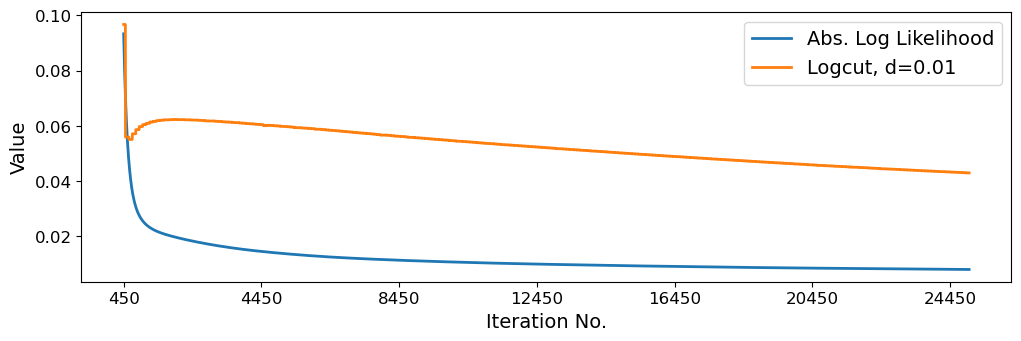
\includegraphics[width=1.0\linewidth]{images/distance/distance_squirrel_ieclam.png}
  %     \caption{Likelihood vs Log Cut Distance comparison}
  % \end{figure}

  \end{block}
\begin{block}{Universality Theorem for IeClam}
  \textbf{Theorem:} IeClam (and hence PieClam) is universal with respect to the log cut distance with $O(\epsilon^{-2})$ communities.

 \textbf{BigClam limitation}: Not universal - embedding dimension must depend on number of nodes.
\end{block}

  \begin{block}{PieClam vs BigClam}
    The innovations of Clam methods are summarized in the table below.
 \vspace{1em}
    
 \begin{table}[h]
  \centering
  \renewcommand{\arraystretch}{1.2}
  \resizebox{0.7\textwidth}{!}{%
    \begin{tabular}{|l|c|c|}
      \hline
      \textbf{Model} & \textbf{Generative} & \textbf{Universal} \\
      \hline
      BigClam & X & X \\
      \hline
      PClam & \checkmark & X \\
      \hline
      IeClam & X & \checkmark \\
      \hline
      PieClam & \checkmark & \checkmark \\
      \hline
    \end{tabular}
  }
\end{table}

  \end{block}
\end{column}

\separatorcolumn

\begin{column}{\colwidth}
  \columntitle{Experiments}
  % \begin{block}{Synthetic Data}
    \textbf{1. Prior Reconstruction}

    Sample a graph from a synthetic prior. Reset affiliation features and fit models to learn the prior.
    \begin{figure}
      \begin{minipage}{0.37\textwidth}
        \centering
        \vspace{-0.18em}
        \hspace{1.1em}\textbf{GT}\\%[0.05em]
        % \vspace{1em}
        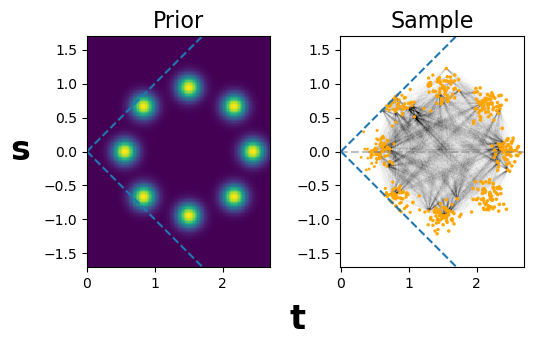
\includegraphics[width=\textwidth]{images/circle/circle_ie_gt.png}
      \end{minipage}
      % \hspace{0.02\textwidth}
      \raisebox{0.5\height}{$\xrightarrow{}$}
      % \hspace{0.02\textwidth}
      \begin{minipage}{0.25\textwidth}
        \centering
        \textbf{Initialize}
        \vspace{0.3em}
        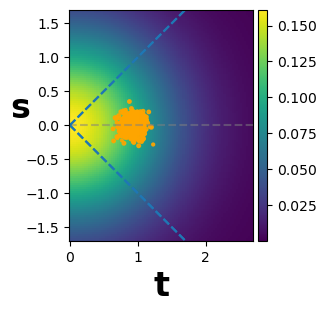
\includegraphics[width=\textwidth]{images/circle/circ_initialization.png}
      \end{minipage}
      % \hspace{0.02\textwidth}
      \raisebox{0.5\height}{$\xrightarrow{}$}
      % \hspace{0.02\textwidth}
      \begin{minipage}{0.25\textwidth}
        \centering
        \textbf{Train}
        \vspace{0.3em}
        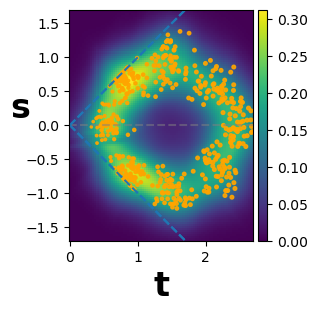
\includegraphics[width=\textwidth]{images/circle/circ_pie_orange_small.png}
      \end{minipage}

      % \begin{minipage}{0.2\textwidth}
     
      % \end{minipage}

      % \hspace{0.1\textwidth}
      % \begin{minipage}{0.2\textwidth}
     
      % \end{minipage}
      % \caption{Node features sampled from synthetic priors and reconstructed with PieClam}
    \end{figure}
    
    \vspace{0.7em}
    
    \textbf{2. SBM Reconstruction}

    Sample edges from an SBM with 3 communities and 9 blocks. And approximate with BigClam and IeClam.
    \begin{figure}[H] 
      % \begin{minipage}{0.2\columnwidth} 
\includegraphics[width=\textwidth]{images/sbm_reconstruction/halfdiag.png} \end{minipage} \hspace{0.5em}
      \begin{minipage}{0.2\columnwidth} 
        \centering
        \textbf{GT}
        \vspace{0.3em}
        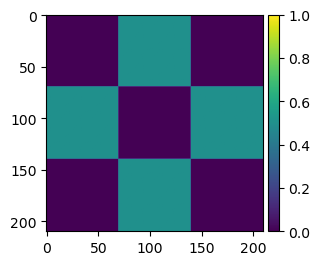
\includegraphics[width=\textwidth]{images/bipart/tripart_gt.png} 
      \end{minipage} \hspace{2em}
      % \begin{minipage}{0.2\columnwidth} 
\includegraphics[width=\textwidth]{images/sbm_reconstruction/halfdiag_pieclam/adj.png} \end{minipage} \hspace{0.5em}
      \begin{minipage}{0.2\columnwidth} 
        \centering
        \textbf{BigClam}
        \vspace{0.3em}
        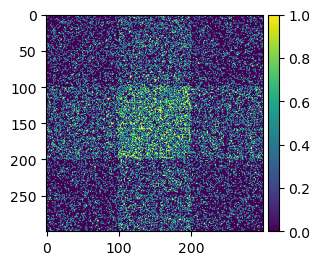
\includegraphics[width=\textwidth]{images/bipart/tripart_bigclam_6comm.png} 
      \end{minipage} \hspace{2em}
      % \begin{minipage}{0.2\columnwidth} 
\includegraphics[width=\textwidth]{images/sbm_reconstruction/halfdiag_pclam/adj.png} \end{minipage}
      \begin{minipage}{0.2\columnwidth} 
        \centering
        \textbf{IeClam}
        \vspace{0.3em}
        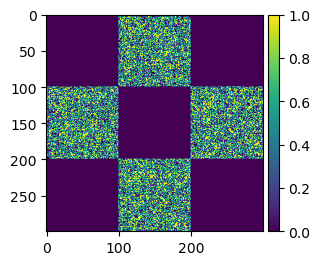
\includegraphics[width=\textwidth]{images/bipart/tripart_ie_4comm.png} 
      \end{minipage} \hspace{0.5em}
      \label{fig:sbm_halfdiag} 
      \end{figure}
      
      \vspace{0.7em}
      
    % \end{block}
    % \begin{block}{Real World Data}
    \textbf{3. Unsupervised Anomaly Detection Results}
    \begin{table}
      \centering
      \small
      \begin{tabular}{|c|c|c|c|}
        \hline
        Method & Reddit & Elliptic & Photo \\
        \hline
        (S)- IeClam & \textbf{64.1} & 43.6 & 57.7 \\
        (S) - PieClam & *64.0 & 43.5 & \underline{59.0} \\
        (P) - PieClam & 46.8 & \textbf{63.2} & 45.7 \\
        (PS) - PieClam & \underline{64.0} & \underline{53.8} & \textbf{59.0} \\
        (S) - BigClam & 63.7 & 43.4 & *58.1 \\
        \hline
        DOMINANT & 51.1 & 29.6 & 51.4 \\
        AnomalyDAE & 50.9 & *49.6 & 50.7 \\
        OCGNN & 52.5 & 25.8 & 53.1 \\
        AEGIS & 53.5 & 45.5 & 55.2 \\
        GAAN & 52.2 & 25.9 & 43.0 \\
        TAM & 60.6 & 40.4 & 56.8 \\
        \hline
      \end{tabular}
      \caption{Anomaly detection AUC scores. First place in \textbf{boldface}, second with \underline{underline}, third with *star.}
    \end{table}

    \vspace{0.7em}

    \textbf{4. Link Prediction Results}
    \begin{table}
      \centering
      \small
      \begin{tabular}{|c|c|c|c|c|}
        \hline
        Method & Squirrel & Photo & Texas & JH55 \\
        \hline
        PieClam & \textbf{98.7} & \textbf{98.4} & \textbf{85.0} & 95.5* \\
        \hline
        BigClam & \underline{98.5} & 97.4* & 78.2* & 94.9 \\
        VGAE & 98.2 & 94.9 & 68.6 & 92.8 \\
        GAT & 98.0 & 97.3 & 68.5 & 94.3 \\
        LINKX & 98.1 & 97.0 & 75.8 & 93.4 \\
        AA & 97.1 & 97.4 & 53.1 & \underline{96.1} \\
        DisenLink & 98.3* & \underline{97.9} & \underline{81.0} & \textbf{97.5} \\
        \hline
      \end{tabular}
      \caption{Link prediction AUC scores. First place in \textbf{boldface}, second with \underline{underline}, third with *star.}
    \end{table}

  % \end{block}
\vspace{-0.5em}
  \columntitle{References}
  % \begin{block}{}
  \vspace{-1em}
    \nocite{yang2013overlapping}
    \nocite{dinh2016density}
    \footnotesize{\bibliographystyle{unsrt}\bibliography{references}}
  % \end{block}

\end{column}

\separatorcolumn
\end{columns}
\end{frame}

\end{document}
